%% ----------------------------------------------------------------
\chapter{Specification}
%% ----------------------------------------------------------------
\label{chap:specification}

\section{Introduction (jc)}

This chapter will describe the brief we were given and an overview of the system and how the elements to be created will sit with the existing components.

The functionality intended for the system is also broken down and the priority given to each task is explained. The things that we should have to give to our customer at the end of the project are also described.

\section{Brief (jc / mitch)}

The original agreed project specification and plan, handed in on the first week of the project, was to design, build, and test an electronic module capable of capturing still images from an unmanned aerial vehicle (UAV) and transmitting the images to a ground station. The module must use the UAV autopilot’s low-bandwidth RS485 serial link (38.4 kBaud). A program must be written to interface with the ground station software over a TCP/IP link, allowing commands to be sent to the electronic module in the UAV and image data to be received and then displayed to the user on the ground. The electronic module should be constructed suitably ruggedly for use in the environment of the UAV.

\section{Block Diagram (jc)}

\begin{figure}[H]
        \centering
        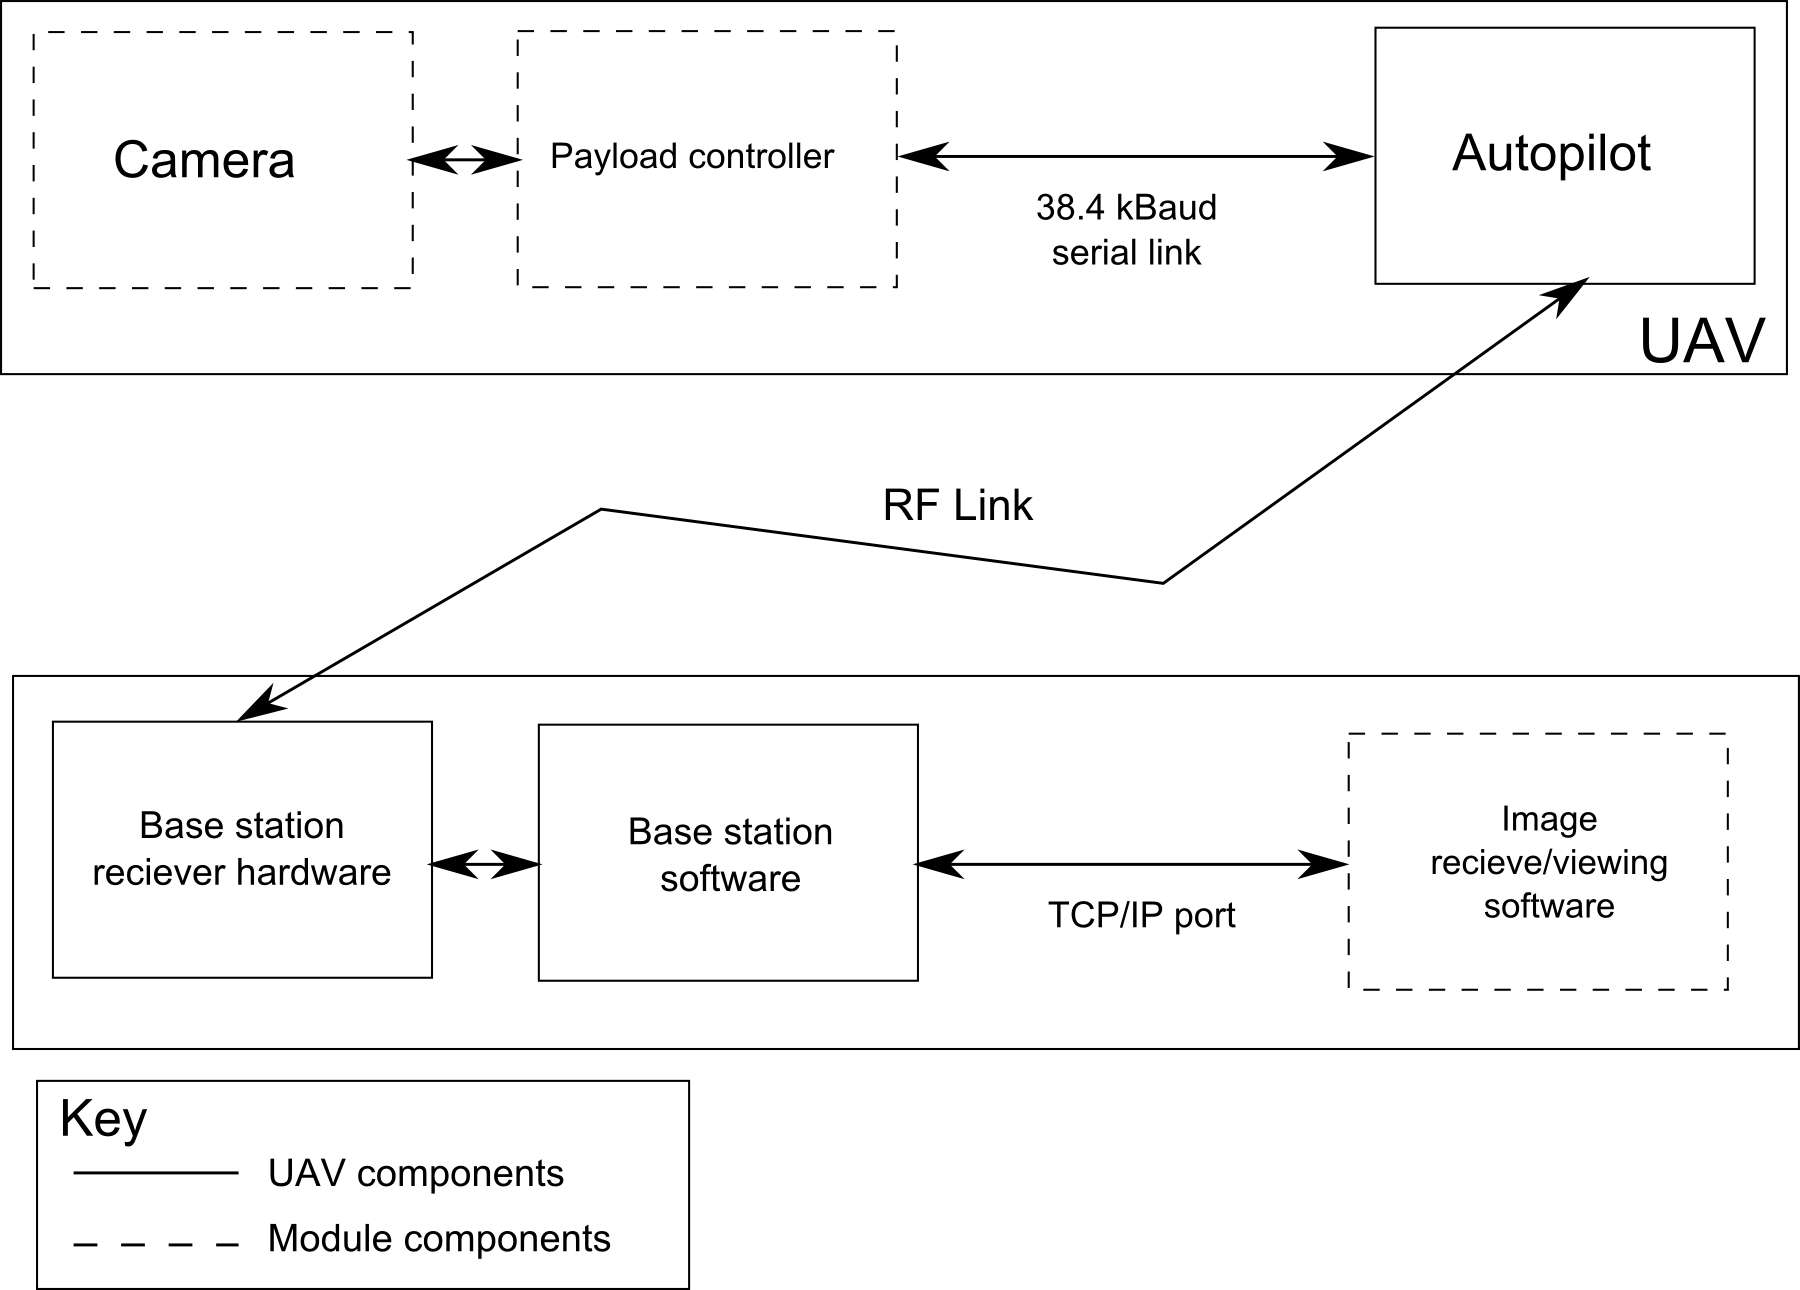
\includegraphics[width=1.00\textwidth]{figures/spec_block_diagram_2.png}
        \captionof{figure}{Block diagram of the specified system}
        \label{fig:block1}
\end{figure}

The above diagram (figure \ref{fig:block1}) gives an overview of how the system described in the specification all comes together. The parts with a solid outline are parts that we were given by our customer to fit our system around. The parts with the dashed outline are the elements of the design that we need to implement ourselves.

Inside the UAV itself will go the camera, the payload controller and the autopilot. The autopilot is provided by our customer and also provides our wireless link to the ground. The camera is simply a camera so that photographs can be taken. The payload controller is the part that needs the most work, it needs to be able to control the camera; take and get images as well as being able to communicate with the autopilot and interpret any commands sent up from the base station (also referred to as the ground station).

On the ground station side of things there is a radio frequency (RF) link (zigBee [] cite []) to the autopilot (simulated by a USB cable for development purposes) which attaches to a computer running the ground station software provided by our customer. The ground station software provides two TCP/IP ports as interfaces, one for sending commands to the ground station software and to the autopilot and one for streaming data from the autopilot. It is these TCP/IP ports that our software on the ground has to interface with so that it can send commands up to the payload controller and then receive and display an image.

\section{Objectives (jc / mitch)} 

The aim of the project was to achieve the following criteria, which were also prioritized in order to ensure organized and efficient work - high priority points are essential or very important to basic system functionality, medium priority points are not essential for basic functionality but help expand the system into a more complete system and low priority points are optional extras that should be added if time permits or if they are very low effort:

	\subsection{The image should be encoded in such a way that a low quality image will be available quickly, the quality of which would improve as more information is downloaded.} \label{sec:spec_a}
This was given a \textbf{high priority} as raw images of an acceptable resolution (see below) contain a large amount of data and we have a slow communications link therefore it would be extremely beneficial to be able to view a low quality image quickly so that you don't have to wait for the full image download to judge its appropriateness.
	\subsection{Minimise the time needed to download the images from the UAV to the base station. The time from the user’s prompt until the image has been fully downloaded will be measured against the theoretical 3 minutes necessary to transmit a full image without using any compression. The goal will be to obtain a full image in \textbf{less than 3 minutes.}} \label{sec:spec_b} 
This 3 minute figure is the time it was calculated it would take to download a raw $640\times480$ 24bit RGB image (approx. 900kB) at 38.4kBaud. This was given a \textbf{high priority} as 3 minutes is a long time to wait for an image to download and downloading images is the point of our system.
	\subsection{The module weight will be \textbf{less than 250g}.} \label{sec:spec_c} 
This was given a \textbf{medium priority} since authough a weight of under 250g would be required for flight, it would be preferable to have a system that is too heavy than one that does not work at all.%as electronics tend not to be very heavy but it is important to bear in mind that the UAV can't carry too much weight.
	\subsection{Image resolution of \textbf{$640\times480$}.} \label{sec:spec_d} 
This was given a \textbf{medium priority}, this value was chosen as a trade off between the amount of data in the image and the quality of the image. Higher resolutions would be acceptable if the download time can be suitable reduced and lower resolutions may also be useful if they are much faster to download.
	\subsection{Allow the user to perform the following actions on the UAV’s camera from the base station:} 
		\subsubsection{Prompt the UAV to \textbf{capture and download an image}.} \label{sec:spec_e} 
This was given a \textbf{high priority} as the main aim of the system is to be able to capture images.
		\subsubsection{\textbf{Cancel} the downloading of any image while the image is being downloaded.} \label{sec:spec_f} 
This was given a \textbf{medium priority} because, given the potentially high download times, a lot of time could be saved by being able to cancel the download of an image you do not want before it has fully downloaded but it is not essential to the basic functionality of the system.
		\subsubsection{\textbf{Resend} an image in case the current preview is corrupted.} \label{sec:spec_g} 
This was given a \textbf{low priority} as it does not affect basic functionality.
		\subsubsection{\textbf{Interrupt} the download of an incomplete image and allow the user to save the incomplete image.} \label{sec:spec_h} 
Please note that this is distinct from the \emph{Cancel} requirement mentioned above since it requires the saving of incomplete images. This was given a \textbf{low priority} as it does not affect basic functionality, but could potentially save the user some time.
		\subsubsection{Select the \textbf{resolution settings} of the image.} \label{sec:spec_i} 
This was given a \textbf{low priority} as it does not affect basic functionality but could be a useful feature for some users.
		\subsubsection{Display a progress indicator which will show the percentage of the image data received, as well as a time estimate for the rest of the image to be downloaded.} \label{sec:spec_j} 
This was given a \textbf{low priority} as it does not affect basic functionality but allows the user to feel more confident that the system is working.
		\subsubsection{The image capture will be triggered automatically by the UAV using triggers built into the autopilot.} \label{sec:spec_k} 
This was given a \textbf{low priority} as it does not affect basic functionality but could be something a user might like to be able to do.
		\subsubsection{Allow the user to command the image capture to \textbf{trigger periodically} over a \textbf{user specified time interval} will be added if time permits.} \label{sec:spec_l} 
This was given a \textbf{low priority} as it does not affect basic functionality but may be a useful feature for some users.
	\subsubsection{Images will be transmitted in \textbf{colour} as opposed to black and white.} \label{sec:spec_m} 
This was given a \textbf{low priority} as black and white images are still useful but colour images would be preferred.
	\subsubsection{The user should be able to select between a colour image and a black and white image.} \label{sec:spec_n} 
This was given a \textbf{low priority} as it does not affect basic functionality.


\section{Deliverables (mitch)}

The deliverables which were planned to be produced by the end of the project and given to the customer include:

	\subsection{\underline{Hardware}:} \label{sec:deliv_hw} Camera module, constructed on PCB (if time permits, otherwise on strip-board),including layout designs.
	\subsection{\underline{Software}:} \label{sec:deliv_sw} All firmware for the electronic module, and software on the base station for viewing images. The full source code and all executable files will be included.
	\subsection{\underline{Documentation}:} \label{sec:deliv_doc} Technical and User Documentation. This includes all schematics related to hardware as well as all other documents concerning both the software and hardware delivered.
	\subsection{\underline{Public repository}:} \label{sec:deliv_git} The full source code, all schematics, and all documents concerning both the software and hardware will be included on a public repository so that the customer may share this information with his clients.

